% TODO
% * mam rozepsat druhou cast dukazu?
%%%%%%%%%%%%%%%%%%%%%%%%%%%%%%%%%%%%%%%%%%%%%%%%%%%%%%%%%%%%%%%%%%%%%%%%%%
\chapter{Hluboký zásobníkový automat s~jedním nevstupním symbolem} \label{kap_deep_pda_fin}


V~této kapitole se zabývám otázkou, jaký je vliv počtu nevstupních symbolů na mocnost hlubokého zásobníkového automatu konečného indexu. V~souvislosti s~touto problematikou představuji hluboký zásobníkový automat s~jedním nevstupním symbolem a porovnávám jej s~programovými gramatikami konečného indexu.

%=========================================================================
\section{Omezení počtu nevstupních symbolů}\label{section_deep_pda_nonterm}


Omezím-li počet nevstupních symbolů hlubokého zásobníkového automatu konečného indexu $M$ na jeden, mohu definovat nový typ automatu $M_\#$. Jestliže chci zachovat sílu automatu $M$, musím být schopna jeho činnost simulovat pomocí $M_\#$. Pro tyto účely zavádím stavy, kde uchovávám informace o~stavu automatu $M$ a o~nevstupních symbolech na zásobníku. To je možné díky konečnému počtu těchto symbolů na zásobníku, neboť jinak by takové řešení vedlo k~nekonečnému počtu stavů. Každé pravidlo pak lze pro každý možný obsah zásobníku převést na jeho ekvivalent nahrazením nevstupních symbolů symbolem $\#$ a jejich uložením do stavu. Převod automatu $M$ na  $M_\#$ popisuji algoritmem \ref{alg_PDA}.

\begin{Alg} \label{alg_PDA}
Převod hlubokého zásobníkového automatu konečného indexu na ekvivalentní s~jedním nevstupním symbolem.

\begin{list}{}{\setlength\parsep{0cm} \setlength\itemsep{0cm} \setlength\leftmargin{1em}}
   \item Vstup: $M = (Q,\Sigma,\Gamma, R, s, S, F, n)$ 
   \item Výstup: $M_\# = (Q_\#,{\Sigma}_\#,{\Gamma}_\#, R_\#, s_\#,  S_\#, F_\#, n)$ \medskip
  
  \item ${\Sigma}_\# := \Sigma$
  \item ${\Gamma}_\# :=\{\#\} \cup \Sigma$
  \item $s_\# := <s,\#>$
  \item $S_\# := \# $ \medskip

  \item Pro každé $mqA \rightarrow pv \in R$, kde $v = b_0 B_1 b_1 B_2 b_2 \dots b_{j-1} B_{j} b_j$, $j \in \{0,1,2,\dots,n-1,n\}$, $b_0,b_i \in {\Sigma}^*$ a $B_i \in (\Gamma - \Sigma)$ pro všechna $i \in \{1,2,\dots,j\}$ : \smallskip

  \subitem A~pro každé $(u,z) \in (\Gamma - \Sigma)^* \times (\Gamma - \Sigma)^*$, kde $|u|=m-1$, $|z|\le n-m$ : \smallskip

  \subsubitem přidej do $Q_\#$ stavy $<q, u~A~z>$, $<p, u~B_1 B_2 \dots B_{j-1} B_{j} z>$,
  \subsubitem přidej do $R_\#$ $m <q, u~A~z> \# \rightarrow <p, u~B_1 B_2 \dots B_{j-1} B_{j} z> b_0 \# b_1 \# b_2 \dots b_{j-1} \# b_j $,
  \subsubitem pokud $q \in F$, přidej do $F_\#$ stav $<q, u~A~z>$,
  \subsubitem pokud $p \in F$, přidej do $F_\#$ stav $<p, u~B_1 B_2 \dots B_{j-1} B_{j} z>$.

\end{list}
\end{Alg}

Je zřejmé, že každý hluboký zásobníkový automat konečného indexu s~jedním nevstupním symbolem splňuje definici pro obecný hluboký zásobníkový automat konečného indexu. Tudíž spolu s~algoritmem \ref{alg_PDA} jsem neformálně dokázala, že tyto automaty jsou ekvivalentní.

\begin{figure}[ht]
\centering
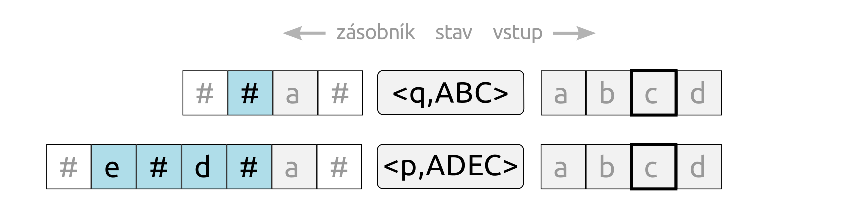
\includegraphics{img/bp_pda03.eps} \bigskip \\
\caption{Aplikace pravidla $2 q B \rightarrow p DdEe$ upraveného podle algoritmu \ref{alg_PDA}.}
\end{figure}

%=========================================================================
\section{Ekvivalence s~programovými gramatikami konečného\\indexu}

A. Meduna \cite{Meduna:FinitelyDeepPDA} dokázal, že hluboké zásobníkové automaty konečného indexu jsou ekvivalentní s~maticovými gramatikami konečného indexu, tudíž třídy jazyků, které zásobníkový automat přijímá, tvoří nekonečnou hierarchii. Vzhledem k~výsledkům v~kapitole \ref{section_deep_pda_nonterm} lze očekávat, že tato vlastnost automatu zůstane i při omezení počtu nevstupních symbolů. Konstrukci důkazu tohoto tvrzení ukážu na ekvivalenci s~programovými gramatikami, přičemž platí, že maticové a programové gramatiky konečného indexu generují stejný jazyk \cite{Dassow:RegulatedRewriting}.

Pro hluboký zásobníkový automat podle článku \cite{Meduna:FinitelyDeepPDA} platí, že jestliže přijme nějaké slovo $w$, pak existuje taková sekvence přechodů přijímající slovo $w$, která provádí pouze pop operace po první pop operaci. Toto tvrzení využiji v~následujícím důkazu, neboť zásobníkový automat, na kterém probíhají jen expanze, funguje jako gramatika. Stačí proto ukázat, že automat je schopen na svém zásobníku simulovat všechny derivace gramatiky a gramatika je schopná simulovat automat.

V~algoritmu \ref{alg_PG} popisuji konstrukci hlubokého zásobníkového automatu konečného indexu s~jedním nevstupním symbolem $M$ simulujícího programovou gramatiku konečného indexu $G$. Stav automatu se v~tomto případě skládá ze dvou položek: označení pravidla, které se bude simulovat v~dalším kroku, a řetězce neterminálů, které jsou na zásobníku nahrazené symbolem $\#$. Automat přejde do koncového stavu, pokud jeho zásobník neobsahuje žádné nevstupní symboly.
 %%%

\begin{Alg} \label{alg_PG}
Převod programové gramatiky konečného indexu na ekvivalentní hluboký zásobníkový automat konečného indexu s~jedním nevstupním symbolem.

\begin{list}{}{\setlength\parsep{0cm} \setlength\itemsep{0cm} \setlength\leftmargin{1em}}
  \item Vstup: $G = (T \cup N ,T,P,S)$ konečného indexu $n$
  \item Výstup: $M = (Q,\Sigma,\Gamma, R, s, S~, F, n)$ \medskip
  
  \item ${\Sigma} := T$
  \item ${\Gamma} := T \cup \{\#\}$
  \item $s_\# := <\sigma>$
  \item $S_\# := \# $ \medskip

  \item Pro každé $p: S~\rightarrow v, g(p) \in P$: 
  \subitem přidej do $R$ pravidlo $<\sigma>_1 \# \rightarrow <p, S> \#$ a do $Q$ stav $<p, S>$. \medskip

  \item Pro každé $q \in (Q \cup \{\varepsilon\})$: 
  \subitem přidej do $F$ stav $<q, \varepsilon>$. \medskip

  \item Pro každé $p: A~\rightarrow v, g(p) \in P$,  kde $v=b_0 B_1 b_1 B_2 b_2 \dots b_{j-1} B_{j} b_j$, $j \in \{0,1,2,3,\dots,n\}$, $b_0,b_i \in T^*$ a $B_i \in N$ pro všechna $i \in \{1,2,\dots,j\}$ : \medskip
  \subitem Pro každé $(k,u,z) \in \{1,2,3,\dots,n-j+1\} \times N^* \times N^*$, kde $|u| = k-1$, $|z|  \le n-k$ : \medskip
  \subsubitem Pokud $g(p) = \emptyset$ :
  \subsubitem přidej do $Q$ stavy $<p,uAz>$, $<\varepsilon, u~B_1 B_2 \dots B_{j-1} B_{j} z>$,
  \subsubitem přidej do $R$ pravidlo :
  \subsubitem $<p,uAz>_k \# \rightarrow <\varepsilon, u~B_1 B_2 \dots B_{j-1} B_{j} z> b_0 \# b_1 \# b_2 \dots b_{j-1} \# b_j$.\medskip
  \subsubitem Jinak pro každé $q \in g(p)$:
  \subsubitem přidej do $Q$ stavy $<p,uAz>$, $<q, u~B_1 B_2 \dots B_{j-1} B_{j} z>$,
  \subsubitem přidej do $R$ pravidlo :
  \subsubitem $<p,uAz>_k \# \rightarrow <q, u~B_1 B_2 \dots B_{j-1} B_{j} z> b_0 \# b_1 \# b_2 \dots b_{j-1} \# b_j$.

\end{list}
\end{Alg}


% TODO rozepsat?

Pro konstrukci důkazu o~převodu hlubokého zásobníkového automatu konečného indexu s~jedním nevstupním symbolem na programovou gramatiku konečného indexu lze beze změny použít postup z~článku \cite{Krivka:RewritingSystems}, který srovnává programové gramatiky s~\#-Rewriting Systems. Programová gramatika simuluje každý krok zásobníkového automatu sekvencí několika derivací. Neterminály obsahují informace o~stavu zásobníku $p$, aktuální pozici výskytu symbolu \# $i$ a celkovém počtu symbolů \# $h$ ve formě zápisu $<p,i,h>$. Simulace aplikace pravidla s~hloubkou expanze $n$ probíhá následovně:

\begin{enumerate}
\item Ve všech neterminálech se aktualizuje jejich pozice a celkový počet symbolů \# vzhledem k~výsledné konfiguraci simulovaného automatu. Symboly se expandují postupně zleva doprava tak, že po každé expanzi se vybere pravidlo pro následující neterminál. 
\item Podle simulovaného pravidla se expanduje neterminál na pozici $n$. Pozice neterminálů za tímto symbolem se v~kroku 1 upravily tak, aby nové neterminály vyplnily chybějící pozice.
\item Neterminály se postupně prochází zleva doprava a pomocný stav se přepisuje stavem aktuálním. Po tomto kroku je simulace dokončena a celý postup se může opakovat.
\end{enumerate}

Tím jsem ukázala, že výše zavedený typ zásobníkového automatu je ekvivalentní s~programovými gramatikami konečného indexu. Z~toho vyplývá, že rodina jazyků přijímaná tímto automatem tvoří nekonečnou hierarchii vycházející z~konečných programových gramatik.


%=========================================================================
